\documentclass[a4paper, 10pt] {article}
\usepackage{tikz}
\usepackage[margin = 1cm]{geometry}
\usepackage{xcolor}
\definecolor{customcolor1}{HTML}{abe0f9}
\definecolor{customcolor2}{HTML}{fee4b3}
\definecolor{customcolor3}{HTML}{00aeef}
\definecolor{customcolor4}{HTML}{f58220}

\title{Data Structure}
\author{Pranto}
\date{\today}

\begin{document}
\maketitle
\section{Graph 5}
Lets Make the Graph of ED task 5.
\begin{center}
\vspace{10pt}
% 1st
\begin{minipage}[t]{.3\linewidth}
    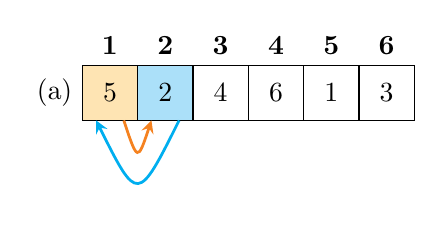
\begin{tikzpicture}
        % Nodes
        \node (a) at (0, 0) {(a)};
        % \node [draw, rectangle, minimum width = 3cm, minimum height = 1cm] (b) at (3, 0.3) {};
        \node [ fill = customcolor2, draw, rectangle, minimum width = 20pt, minimum height = 20pt] (b) at (20pt, 0pt) {5};
        \node [ fill = customcolor1, draw, rectangle, minimum width = 20pt, minimum height = 20pt] (c) at (40pt, 0pt) {2};
        \node [ draw, rectangle, minimum width = 20pt, minimum height = 20pt] (d) at (60pt, 0pt) {4};
        \node [ draw, rectangle, minimum width = 20pt, minimum height = 20pt] (e) at (80pt, 0pt) {6};
        \node [ draw, rectangle, minimum width = 20pt, minimum height = 20pt] (f) at (100pt, 0pt) {1};
        \node [ draw, rectangle, minimum width = 20pt, minimum height = 20pt] (g) at (120pt, 0pt) {3};

        % Draw the links
        \draw [->, > = stealth, line width = 1pt, color = customcolor3] (45pt, -10pt) .. controls(30pt, -40pt) .. (15pt, -10pt);      
        \draw [->, > = stealth, line width = 1pt, color = customcolor4] (25pt, -10pt) .. controls(30pt, -25pt) .. (35pt, -10pt);      
        
        % Node Level
        \node [above] at (b.north) {\textbf{1}};
        \node [above] at (c.north) {\textbf{2}};
        \node [above] at (d.north) {\textbf{3}};
        \node [above] at (e.north) {\textbf{4}};
        \node [above] at (f.north) {\textbf{5}};
        \node [above] at (g.north) {\textbf{6}};

    \end{tikzpicture}
\end{minipage}
% 2nd
\begin{minipage}[t]{.3\linewidth}
    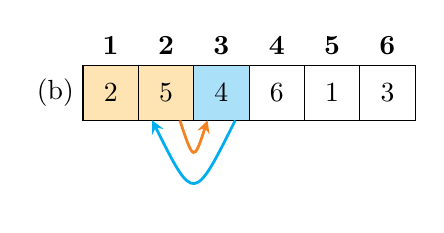
\begin{tikzpicture}
        % Nodes
        \node (a) at (0, 0) {(b)};
        % \node [draw, rectangle, minimum width = 3cm, minimum height = 1cm] (b) at (3, 0.3) {};
        \node [fill = customcolor2, draw, rectangle, minimum width = 20pt, minimum height = 20pt] (c) at (40pt, 0pt) {5};
        \node [fill = customcolor2, draw, rectangle, minimum width = 20pt, minimum height = 20pt] (b) at (20pt, 0pt) {2};
        \node [fill = customcolor1, draw, rectangle, minimum width = 20pt, minimum height = 20pt] (d) at (60pt, 0pt) {4};
        \node [ draw, rectangle, minimum width = 20pt, minimum height = 20pt] (e) at (80pt, 0pt) {6};
        \node [ draw, rectangle, minimum width = 20pt, minimum height = 20pt] (f) at (100pt, 0pt) {1};
        \node [ draw, rectangle, minimum width = 20pt, minimum height = 20pt] (g) at (120pt, 0pt) {3};

        % Draw the links
        \draw [->, > = stealth, line width = 1pt, customcolor3] (65pt, -10pt) .. controls(50pt, -40pt) .. (35pt, -10pt);      
        \draw [->, > = stealth, line width = 1pt, customcolor4] (45pt, -10pt) .. controls(50pt, -25pt) .. (55pt, -10pt);      
        
        % Node Level
        \node [above] at (b.north) {\textbf{1}};
        \node [above] at (c.north) {\textbf{2}};
        \node [above] at (d.north) {\textbf{3}};
        \node [above] at (e.north) {\textbf{4}};
        \node [above] at (f.north) {\textbf{5}};
        \node [above] at (g.north) {\textbf{6}};

    \end{tikzpicture}
\end{minipage}
% 3rd
\begin{minipage}[t]{.3\linewidth}
    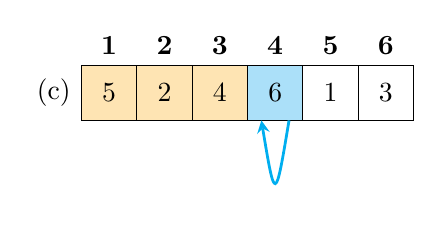
\begin{tikzpicture}
        % Nodes
        \node (a) at (0, 0) {(c)};
        % \node [draw, rectangle, minimum width = 3cm, minimum height = 1cm] (b) at (3, 0.3) {};
        \node [fill = customcolor2, draw, rectangle, minimum width = 20pt, minimum height = 20pt] (b) at (20pt, 0pt) {5};
        \node [fill = customcolor2, draw, rectangle, minimum width = 20pt, minimum height = 20pt] (c) at (40pt, 0pt) {2};
        \node [fill = customcolor2, draw, rectangle, minimum width = 20pt, minimum height = 20pt] (d) at (60pt, 0pt) {4};
        \node [fill = customcolor1, draw, rectangle, minimum width = 20pt, minimum height = 20pt] (e) at (80pt, 0pt) {6};
        \node [ draw, rectangle, minimum width = 20pt, minimum height = 20pt] (f) at (100pt, 0pt) {1};
        \node [ draw, rectangle, minimum width = 20pt, minimum height = 20pt] (g) at (120pt, 0pt) {3};

        % Draw the links
        \draw [->, > = stealth, line width = 1pt, color = customcolor3] (85pt, -10pt) .. controls(80pt, -40pt) .. (75pt, -10pt);      
        
        % Node Level
        \node [above] at (b.north) {\textbf{1}};
        \node [above] at (c.north) {\textbf{2}};
        \node [above] at (d.north) {\textbf{3}};
        \node [above] at (e.north) {\textbf{4}};
        \node [above] at (f.north) {\textbf{5}};
        \node [above] at (g.north) {\textbf{6}};

    \end{tikzpicture}
\end{minipage}   
\vspace{40pt}
% 4th
\begin{minipage}[t]{.3\linewidth}
    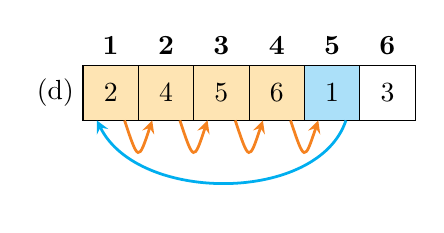
\begin{tikzpicture}
        % Nodes
        \node (a) at (0, 0) {(d)};
        % \node [draw, rectangle, minimum width = 3cm, minimum height = 1cm] (b) at (3, 0.3) {};
        \node [fill = customcolor2, draw, rectangle, minimum width = 20pt, minimum height = 20pt] (b) at (20pt, 0pt) {2};
        \node [fill = customcolor2, draw, rectangle, minimum width = 20pt, minimum height = 20pt] (c) at (40pt, 0pt) {4};
        \node [fill = customcolor2, draw, rectangle, minimum width = 20pt, minimum height = 20pt] (d) at (60pt, 0pt) {5};
        \node [fill = customcolor2, draw, rectangle, minimum width = 20pt, minimum height = 20pt] (e) at (80pt, 0pt) {6};
        \node [fill = customcolor1, draw, rectangle, minimum width = 20pt, minimum height = 20pt] (f) at (100pt, 0pt) {1};
        \node [ draw, rectangle, minimum width = 20pt, minimum height = 20pt] (g) at (120pt, 0pt) {3};

        % Draw the links
        \draw [->, > = stealth, line width = 1pt, color = customcolor3] (105pt, -10pt) .. controls(95pt, -40pt) and (30pt, -40pt) .. (15pt, -10pt);      
        \draw [->, > = stealth, line width = 1pt, color = customcolor4] (25pt, -10pt) .. controls(30pt, -25pt) .. (35pt, -10pt);      
        \draw [->, > = stealth, line width = 1pt, color = customcolor4] (45pt, -10pt) .. controls(50pt, -25pt) .. (55pt, -10pt);      
        \draw [->, > = stealth, line width = 1pt, color = customcolor4] (65pt, -10pt) .. controls(70pt, -25pt) .. (75pt, -10pt);      
        \draw [->, > = stealth, line width = 1pt, color = customcolor4] (85pt, -10pt) .. controls(90pt, -25pt) .. (95pt, -10pt);      
          
        % Node Level
        \node [above] at (b.north) {\textbf{1}};
        \node [above] at (c.north) {\textbf{2}};
        \node [above] at (d.north) {\textbf{3}};
        \node [above] at (e.north) {\textbf{4}};
        \node [above] at (f.north) {\textbf{5}};
        \node [above] at (g.north) {\textbf{6}};

    \end{tikzpicture}
\end{minipage}
% 5th
\begin{minipage}[t]{.3\linewidth}
    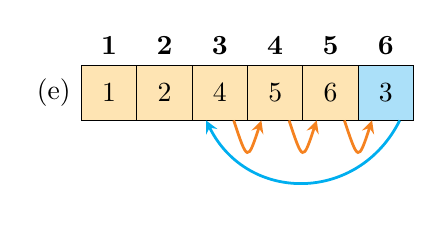
\begin{tikzpicture}
        % Nodes
        \node (a) at (0, 0) {(e)};
        % \node [draw, rectangle, minimum width = 3cm, minimum height = 1cm] (b) at (3, 0.3) {};
        \node [fill = customcolor2, draw, rectangle, minimum width = 20pt, minimum height = 20pt] (b) at (20pt, 0pt) {1};
        \node [fill = customcolor2, draw, rectangle, minimum width = 20pt, minimum height = 20pt] (c) at (40pt, 0pt) {2};
        \node [fill = customcolor2, draw, rectangle, minimum width = 20pt, minimum height = 20pt] (d) at (60pt, 0pt) {4};
        \node [fill = customcolor2, draw, rectangle, minimum width = 20pt, minimum height = 20pt] (e) at (80pt, 0pt) {5};
        \node [fill = customcolor2, draw, rectangle, minimum width = 20pt, minimum height = 20pt] (f) at (100pt, 0pt) {6};
        \node [fill = customcolor1, draw, rectangle, minimum width = 20pt, minimum height = 20pt] (g) at (120pt, 0pt) {3};

        % Draw the links
        \draw [->, > = stealth, line width = 1pt, color = customcolor3] (125pt, -10pt) .. controls(110pt, -40pt) and (70pt, -40pt) .. (55pt, -10pt);      
        \draw [->, > = stealth, line width = 1pt, color = customcolor4] (65pt, -10pt) .. controls(70pt, -25pt) .. (75pt, -10pt);      
        \draw [->, > = stealth, line width = 1pt, color = customcolor4] (85pt, -10pt) .. controls(90pt, -25pt) .. (95pt, -10pt);      
        \draw [->, > = stealth, line width = 1pt, color = customcolor4] (105pt, -10pt) .. controls(110pt, -25pt) .. (115pt, -10pt);      
        
        % Node Level
        \node [above] at (b.north) {\textbf{1}};
        \node [above] at (c.north) {\textbf{2}};
        \node [above] at (d.north) {\textbf{3}};
        \node [above] at (e.north) {\textbf{4}};
        \node [above] at (f.north) {\textbf{5}};
        \node [above] at (g.north) {\textbf{6}};

    \end{tikzpicture}
\end{minipage}
% 6th
\begin{minipage}[t]{0.3\linewidth}
    \vspace{-64pt}
    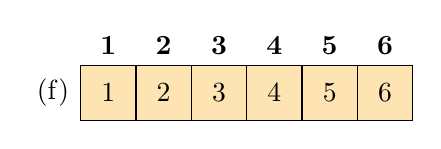
\begin{tikzpicture}
        % Nodes
        \node (a) at (0, 0) {(f)};
        % \node [draw, rectangle, minimum width = 3cm, minimum height = 1cm] (b) at (3, 0.3) {};
        \node [fill = customcolor2, draw, rectangle, minimum width = 20pt, minimum height = 20pt] (b) at (20pt, 0pt) {1};
        \node [fill = customcolor2, draw, rectangle, minimum width = 20pt, minimum height = 20pt] (c) at (40pt, 0pt) {2};
        \node [fill = customcolor2, draw, rectangle, minimum width = 20pt, minimum height = 20pt] (d) at (60pt, 0pt) {3};
        \node [fill = customcolor2, draw, rectangle, minimum width = 20pt, minimum height = 20pt] (e) at (80pt, 0pt) {4};
        \node [fill = customcolor2, draw, rectangle, minimum width = 20pt, minimum height = 20pt] (f) at (100pt, 0pt) {5};
        \node [fill = customcolor2, draw, rectangle, minimum width = 20pt, minimum height = 20pt] (g) at (120pt, 0pt) {6};
        
        % Draw the links
        % \draw [->, > = stealth, line width = 1pt, rounded corners = 5pt] (15pt, -10pt) .. controls(30pt, -40pt) .. (45pt, -10pt);           
        % \draw [->, > = stealth, line width = 1pt, rounded corners = 5pt] (35pt, -10pt) .. controls(30pt, -25pt) .. (25pt, -10pt); 
        
        % Node Level
        \node [above] at (b.north) {\textbf{1}};
        \node [above] at (c.north) {\textbf{2}};
        \node [above] at (d.north) {\textbf{3}};
        \node [above] at (e.north) {\textbf{4}};
        \node [above] at (f.north) {\textbf{5}};
        \node [above] at (g.north) {\textbf{6}};

    \end{tikzpicture}
\end{minipage}
\end{center} 
\end{document}
